\documentclass[11pt,letterpaper]{article}
\usepackage[margin=1in]{geometry}
\usepackage[T1]{fontenc}
\usepackage{newtxtext,newtxmath}
\usepackage{graphicx,booktabs,xcolor,amsmath,microtype,tikz,enumitem,caption,array}
\usepackage[hidelinks]{hyperref}
\usetikzlibrary{positioning,fit,arrows.meta,calc,backgrounds,decorations.pathreplacing}
\captionsetup{font=small,labelfont=bf}
\setlist{itemsep=2pt,topsep=4pt,leftmargin=1.4em}
\setlength{\parskip}{4pt}
\emergencystretch=2em
\definecolor{cblue}{HTML}{2a78d6}
\definecolor{corange}{HTML}{eb6834}
\definecolor{caqua}{HTML}{1baf7a}
\definecolor{cpurple}{HTML}{8c5bd6}
\definecolor{cgray}{HTML}{8a8984}
\newcommand{\code}[1]{\texttt{\small #1}}
\newcommand{\shape}[1]{\texttt{\footnotesize[#1]}}
\tikzset{
  arr/.style={-{Stealth[length=5pt]},draw=black!60,thick},
  box/.style={draw=#1!80!black,fill=#1!10,rounded corners=2pt,inner sep=4pt,align=center},
  box/.default=cgray,
}

\title{\Large\bfseries How WheelNet Works\\[2pt]\large A step-by-step guide to the architecture}
\author{Companion to \emph{Will It Wheel? Predicting Which Passed Cards Come Back}}
\date{\small October 2026}

\begin{document}
\maketitle

\noindent The paper's Figure~1 squeezes the whole model into five boxes. This guide unpacks them one at a
time. It assumes you know how a booster draft works and roughly what a neural network is (a function with
lots of tunable numbers, fitted by gradient descent). It does not assume you know transformers. Every
claim about the model refers to the code in \code{src/openlane/nn.py}, and the sizes are those of the
shipped MSH model (\code{results/MSH.PremierDraft/models/wheelnet\_time.pt}). WheelNet is a sibling of
PickNet, and this guide follows the PickNet guide's structure; Section~\ref{sec:vs} lists the differences.

{\small\setlength{\parskip}{0pt}\tableofcontents}

% =====================================================================
\section{The job, and the big picture}

Every time a drafter passes a pack early in a round, WheelNet looks at everything they could have known at
that moment and outputs, for \emph{each} card they passed, a probability that it comes back eight picks
later: ``Hex Magic 88\%, Super Suit 50\%, Jessica Jones 7\%, \ldots''. It is trained to make those
probabilities honest: of the cards it gives 30\%, about 30\% should come back.

The model has two halves, and almost everything else is plumbing around them:

\begin{enumerate}
\item \textbf{The history encoder} reads the draft so far, one token per pick, and produces a \emph{state}
for each pick: a list of 192 numbers that summarises ``what this drafter has seen and done so far'': the
packs they were shown, the cards they took, and what the rest of the table took from the packs that came
back.
\item \textbf{The pack decoder} takes the cards the drafter just passed, lets them look at each other and at
the history, and gives each card a score. A sigmoid turns each score into a probability.
\end{enumerate}

\begin{figure}[!htbp]
\centering
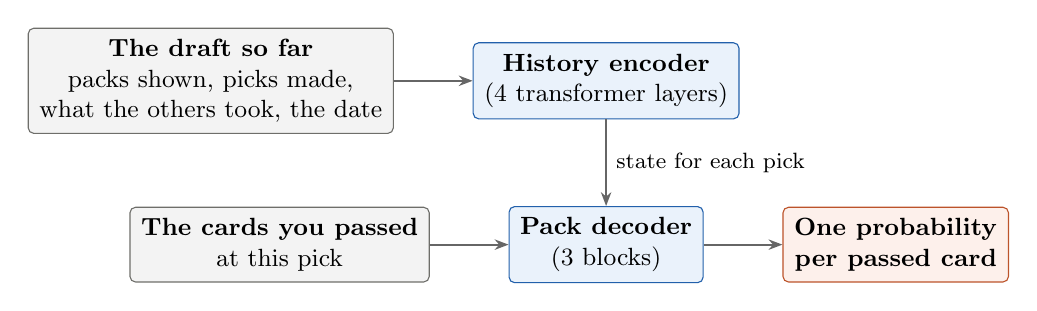
\begin{tikzpicture}[font=\small,node distance=0.55cm]
\node[box] (data) {\textbf{The draft so far}\\packs shown, picks made,\\what the others took, the date};
\node[box=cblue,right=1.0cm of data] (hist) {\textbf{History encoder}\\(4 transformer layers)};
\node[box=cblue,below=1.1cm of hist] (dec) {\textbf{Pack decoder}\\(3 blocks)};
\node[box,left=1.0cm of dec] (pack) {\textbf{The cards you passed}\\at this pick};
\node[box=corange,right=1.0cm of dec] (out) {\textbf{One probability}\\\textbf{per passed card}};
\draw[arr] (data) -- (hist);
\draw[arr] (hist) -- node[right,font=\footnotesize]{state for each pick} (dec);
\draw[arr] (pack) -- (dec);
\draw[arr] (dec) -- (out);
\end{tikzpicture}
\caption{The model at the coarsest level.}
\label{fig:big}
\end{figure}

\noindent A useful way to think about it: the history encoder answers ``what do I know about this table
right now?'' and the pack decoder answers ``given that, which of the cards I just passed will the next
seven drafters leave alone, considering what else they could take instead?''.

Figure~\ref{fig:full} (page~\pageref{fig:full}) is the same model with nothing left out: every layer that has
trained weights, how many weights each one has, and the shape of every tensor for one draft. \textbf{Blue}
boxes have trained weights; the small blue number is how many. \textbf{Grey} boxes are data, \textbf{white}
boxes are fixed operations with no weights, $\oplus$ adds vectors, and {\color{corange}$\blacklozenge$} marks a
lookup in the card table. Shapes are per draft (a batch adds a leading $B$) for MSH's 14-card packs. The
history-encoder layer is stacked 4 times and the pack-decoder block 3 times, each copy with its own weights;
the thin grey lines that skip around each attention and MLP are the residual connections. Every decoder block
reads the same history states $\mathbf h$. Dropout (0.2) after each attention and MLP is not drawn. The counts
add up to 3,864,001. The rest of this guide walks through the figure from top to bottom.

\begin{figure}[p]
\centering
\resizebox{!}{0.94\textheight}{% Every learned layer of WheelNet for one MSH draft (wheelnet_time). \input by architecture.tex.
{\def\fT{\fontsize{5}{6}\selectfont}\def\fS{\fontsize{7}{8}\selectfont}\def\fF{\fontsize{8}{9.5}\selectfont}
\def\fN{\fontsize{10}{12}\selectfont}\def\fL{\fontsize{12}{14}\selectfont}
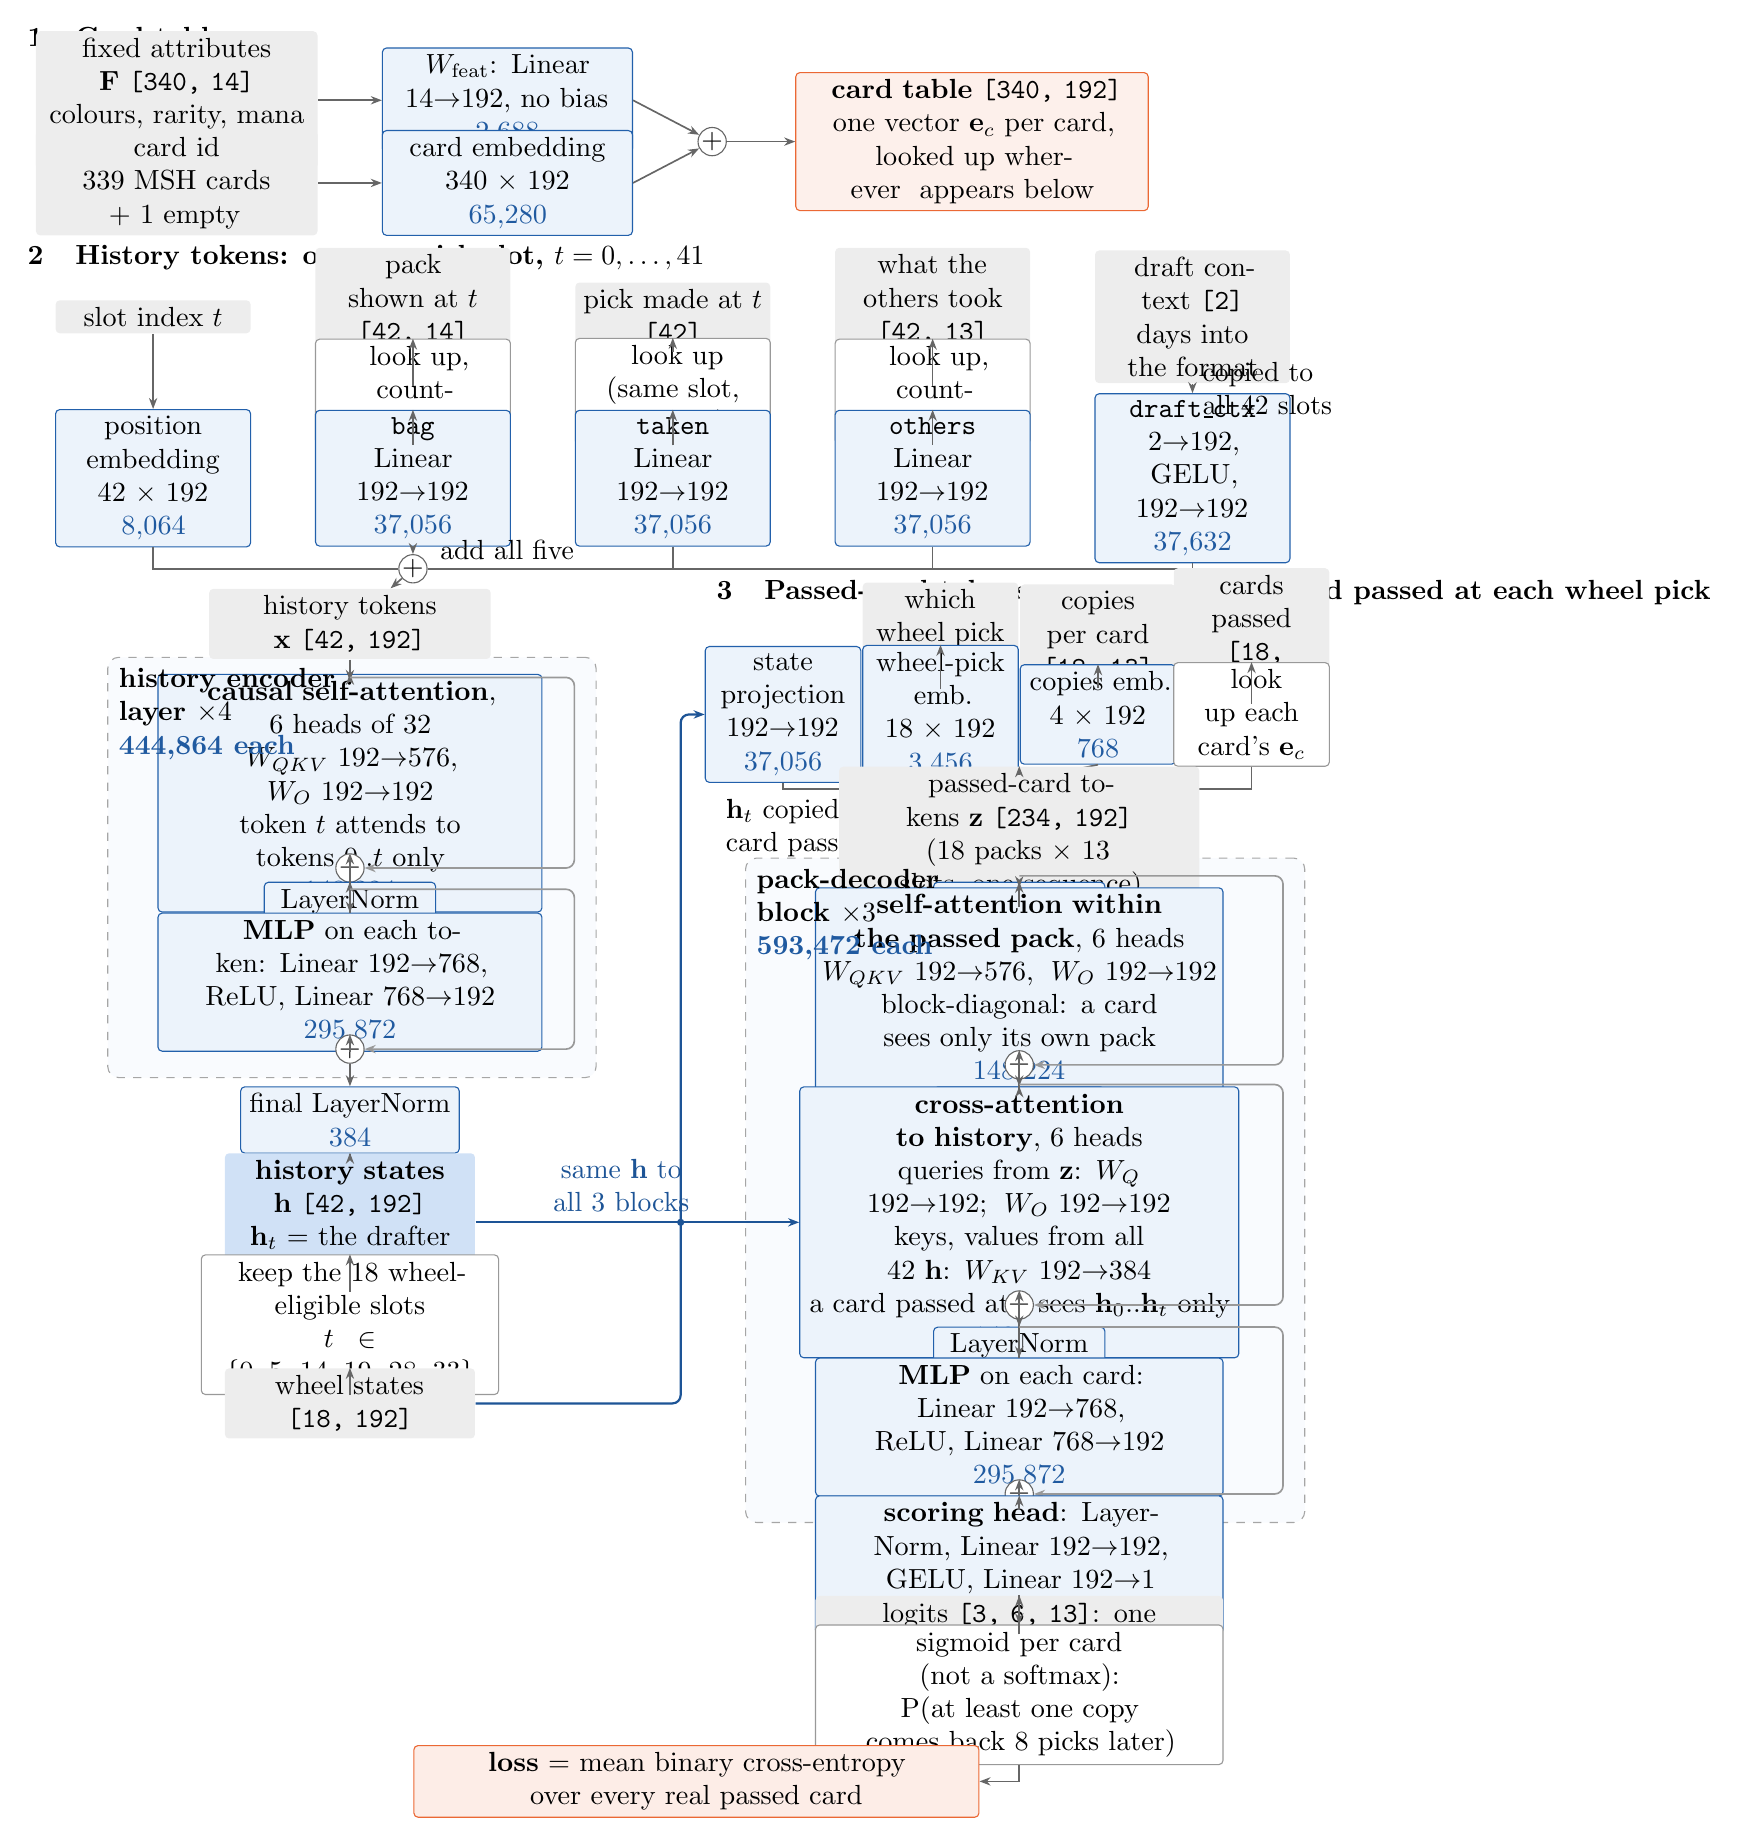
\begin{tikzpicture}[
  font=\fS,
  L/.style={draw=cblue!80!black,fill=cblue!9,rounded corners=1.5pt,align=center,inner sep=2.5pt,text width=#1},
  L/.default=2.3cm,
  O/.style={draw=black!40,fill=white,rounded corners=1.5pt,align=center,inner sep=2.5pt,text width=#1},
  O/.default=2.3cm,
  T/.style={fill=black!7,rounded corners=1.5pt,align=center,inner sep=2.5pt,text width=#1},
  T/.default=2.3cm,
  plus/.style={circle,draw=black!60,fill=white,inner sep=0pt,minimum size=3.4mm,font=\fF},
  a/.style={-{Stealth[length=4pt]},draw=black!60,semithick},
  ln/.style={draw=black!60,semithick},
  res/.style={-{Stealth[length=4pt]},draw=black!40,semithick,rounded corners=3pt},
  hb/.style={-{Stealth[length=4pt]},draw=cblue!70!black,thick,rounded corners=3pt},
  grp/.style={draw=black!35,dashed,rounded corners=4pt,inner sep=5pt},
  hd/.style={font=\fF\bfseries,anchor=west,inner sep=0pt},
  gl/.style={font=\fS\bfseries,anchor=north west,inner sep=0pt,align=left},
]
\def\pn#1{\\{\fT\color{cblue!75!black}#1}}
\def\shape#1{{\ttfamily[#1]}}
\def\lk{{\color{corange}$\blacklozenge$}}

% ------------------------------------------------------------ 1. card table
\node[hd] at (0,0) {1\quad Card table};
\node[T=3.4cm] (F) at (1.9,-0.8) {fixed attributes $\mathbf F$ \shape{340, 14}\\colours, rarity, mana value, creature, bonus};
\node[L=3.0cm] (WF) at (6.1,-0.8) {$W_{\text{feat}}$: Linear 14$\to$192, no bias\pn{2,688}};
\node[T=3.4cm] (NID) at (1.9,-1.85) {card id\\339 MSH cards + 1 empty};
\node[L=3.0cm] (NE) at (6.1,-1.85) {card embedding\\340 $\times$ 192\pn{65,280}};
\node[plus] (pa) at (8.7,-1.325) {+};
\node[T=4.3cm,draw=corange,fill=corange!10] (TAB) at (12.0,-1.325)
  {\lk\ \textbf{card table} \shape{340, 192}\\one vector $\mathbf e_c$ per card,\\looked up wherever \lk\ appears below};
\draw[a] (F) -- (WF);
\draw[a] (NID) -- (NE);
\draw[a] (WF.east) -- (pa);
\draw[a] (NE.east) -- (pa);
\draw[a] (pa) -- (TAB);

% ------------------------------------------------------------ 2. history tokens
\node[hd] at (0,-2.8) {2\quad History tokens: one per pick slot, $t = 0,\dots,41$};
\foreach \k/\x in {1/1.6,2/4.9,3/8.2,4/11.5,5/14.8} \coordinate (c\k) at (\x,0);
\node[T] (i1) at (c1|-0,-3.55) {slot index $t$};
\node[T] (i2) at (c2|-0,-3.55) {pack shown at $t$\\\shape{42, 14} ids + copies};
\node[T] (i3) at (c3|-0,-3.55) {pick made at $t$\\\shape{42}};
\node[T] (i4) at (c4|-0,-3.55) {what the others took\\\shape{42, 13} ids + copies};
\node[T] (i5) at (c5|-0,-3.55) {draft context \shape{2}\\days into the format};
\node[O] (o2) at (c2|-0,-4.5) {\lk\ look up,\\count-weighted mean};
\node[O] (o3) at (c3|-0,-4.5) {\lk\ look up\\(same slot, no shift)};
\node[O] (o4) at (c4|-0,-4.5) {\lk\ look up,\\count-weighted mean};
\node[L] (l1) at (c1|-0,-5.6) {position embedding\\42 $\times$ 192\pn{8,064}};
\node[L] (l2) at (c2|-0,-5.6) {{\ttfamily bag}\\Linear 192$\to$192\pn{37,056}};
\node[L] (l3) at (c3|-0,-5.6) {{\ttfamily taken}\\Linear 192$\to$192\pn{37,056}};
\node[L] (l4) at (c4|-0,-5.6) {{\ttfamily others}\\Linear 192$\to$192\pn{37,056}};
\node[L] (l5) at (c5|-0,-5.6) {{\ttfamily draft\_ctx}\\2$\to$192, GELU, 192$\to$192\pn{37,632}};
\draw[a] (i1) -- (l1);
\foreach \k in {2,3,4} {\draw[a] (i\k) -- (o\k); \draw[a] (o\k) -- (l\k);}
\draw[a] (i5) -- node[right,font=\fT,align=left]{copied to\\all 42 slots} (l5);
\node[plus] (pt) at (c2|-0,-6.75) {+};
\draw[a] (l2) -- (pt);
\draw[ln] (l1.south) |- (pt.west);
\draw[ln] (l5.south) |- (pt.east);
\foreach \k in {3,4} \draw[ln] (l\k.south) -- (l\k.south|-pt.center);
\node[font=\fT,above right=0pt and 1pt] at (pt.east) {add all five};

% ------------------------------------------------------------ 3. history encoder (left column)
\def\xc{4.1}
\node[T=3.4cm] (x) at (\xc,-7.45) {history tokens $\mathbf x$ \shape{42, 192}};
\draw[a] (pt) -- (x);
\node[L=2.0cm] (eln1) at (\xc,-8.6) {LayerNorm\pn{384}};
\node[L=4.7cm] (esa) at (\xc,-9.6) {\textbf{causal self-attention}, 6 heads of 32\\$W_{QKV}$ 192$\to$576,\; $W_O$ 192$\to$192\\token $t$ attends to tokens $0..t$ only\pn{148,224}};
\node[plus] (ep1) at (\xc,-10.55) {+};
\node[L=2.0cm] (eln2) at (\xc,-11.15) {LayerNorm\pn{384}};
\node[L=4.7cm] (emlp) at (\xc,-12.0) {\textbf{MLP} on each token: Linear 192$\to$768,\\ReLU, Linear 768$\to$192\pn{295,872}};
\node[plus] (ep2) at (\xc,-12.85) {+};
\draw[a] (x) -- (eln1); \draw[a] (eln1) -- (esa); \draw[a] (esa) -- (ep1);
\draw[a] (ep1) -- (eln2); \draw[a] (eln2) -- (emlp); \draw[a] (emlp) -- (ep2);
\draw[res] (\xc,-8.13) -| (6.95,-9.0) |- (ep1.east);
\draw[res] (\xc,-10.82) -| (6.95,-11.5) |- (ep2.east);
\begin{scope}[on background layer]
\node[grp,fill=cblue!3,fit={(eln1)(esa)(emlp)(ep2)(7.05,-8.05)(1.2,-8.1)}] (enc) {};
\end{scope}
\node[gl] at ([shift={(4pt,-4pt)}]enc.north west) {history encoder\\layer {\fN$\times 4$}\\\textcolor{cblue!75!black}{\fT 444,864 each}};
\node[L=2.6cm] (fln) at (\xc,-13.75) {final LayerNorm\pn{384}};
\draw[a] (ep2) -- (fln);
\node[T=3.0cm,fill=cblue!22] (h) at (\xc,-15.05) {\textbf{history states} $\mathbf h$ \shape{42, 192}\\$\mathbf h_t$ = the drafter just after pick $t$};
\draw[a] (fln) -- (h);
\node[O=3.6cm] (sel) at (\xc,-16.35) {keep the 18 wheel-eligible slots\\$t \in \{0..5,\,14..19,\,28..33\}$};
\node[T=3.0cm] (hs) at (\xc,-17.35) {wheel states \shape{18, 192}};
\draw[a] (h) -- (sel); \draw[a] (sel) -- (hs);

% ------------------------------------------------------------ 4. passed-card tokens (right column)
\def\xr{12.6}
\node[hd] at (8.75,-7.05) {3\quad Passed-card tokens: one per distinct card passed at each wheel pick};
\node[T=1.8cm] (wpi) at (11.6,-7.6) {which wheel pick\\(0..17)};
\node[T=1.8cm] (ccnt) at (13.6,-7.6) {copies per card\\\shape{18, 13}};
\node[T=1.8cm] (cidx) at (15.55,-7.6) {cards passed\\\shape{18, 13} ids};
\node[L=1.8cm] (sp) at (9.6,-8.6) {state projection\\192$\to$192\pn{37,056}};
\node[L=1.8cm] (wp) at (11.6,-8.6) {wheel-pick emb.\\18 $\times$ 192\pn{3,456}};
\node[L=1.8cm] (cp) at (13.6,-8.6) {copies emb.\\4 $\times$ 192\pn{768}};
\node[O=1.8cm] (clk) at (15.55,-8.6) {\lk\ look up each card's $\mathbf e_c$};
\draw[a] (wpi) -- (wp); \draw[a] (ccnt) -- (cp); \draw[a] (cidx) -- (clk);
\node[plus] (pc) at (\xr,-9.55) {+};
\draw[a] (sp.south) |- (pc.west);
\draw[a] (wp.south) -- (pc.north west);
\draw[a] (cp.south) -- (pc.north east);
\draw[a] (clk.south) |- (pc.east);
\node[font=\fT,align=left,anchor=north west] at (8.75,-9.55) {$\mathbf h_t$ copied to every\\card passed at $t$};
\node[T=4.4cm] (z) at (\xr,-10.15) {passed-card tokens $\mathbf z$ \shape{234, 192}\\(18 packs $\times$ 13 slots, one sequence)};
\draw[a] (pc) -- (z);
\draw[hb] (hs.east) -- (8.3,-17.35) -- (8.3,-8.6) -- (sp.west);
\fill[cblue!70!black] (8.3,-15.05) circle (1.3pt);

% ------------------------------------------------------------ 5. pack decoder (right column)
\node[L=2.0cm] (dln1) at (\xr,-11.15) {LayerNorm\pn{384}};
\node[L=5.0cm] (dsa) at (\xr,-12.1) {\textbf{self-attention within the passed pack}, 6 heads\\$W_{QKV}$ 192$\to$576,\; $W_O$ 192$\to$192\\block-diagonal: a card sees only its own pack\pn{148,224}};
\node[plus] (dp1) at (\xr,-13.05) {+};
\node[L=2.0cm] (dln2) at (\xr,-13.75) {LayerNorm\pn{384}};
\node[L=5.4cm] (dca) at (\xr,-15.05) {\textbf{cross-attention to history}, 6 heads\\queries from $\mathbf z$: $W_Q$ 192$\to$192;\; $W_O$ 192$\to$192\\keys, values from all 42 $\mathbf h$: $W_{KV}$ 192$\to$384\\a card passed at $t$ sees $\mathbf h_0..\mathbf h_t$ only\pn{148,224}};
\node[plus] (dp2) at (\xr,-16.1) {+};
\node[L=2.0cm] (dln3) at (\xr,-16.8) {LayerNorm\pn{384}};
\node[L=5.0cm] (dmlp) at (\xr,-17.65) {\textbf{MLP} on each card: Linear 192$\to$768,\\ReLU, Linear 768$\to$192\pn{295,872}};
\node[plus] (dp3) at (\xr,-18.5) {+};
\draw[a] (z) -- (dln1); \draw[a] (dln1) -- (dsa); \draw[a] (dsa) -- (dp1);
\draw[a] (dp1) -- (dln2); \draw[a] (dln2) -- (dca); \draw[a] (dca) -- (dp2);
\draw[a] (dp2) -- (dln3); \draw[a] (dln3) -- (dmlp); \draw[a] (dmlp) -- (dp3);
\draw[res] (\xr,-10.65) -| (15.95,-11.5) |- (dp1.east);
\draw[res] (\xr,-13.3) -| (15.95,-14.0) |- (dp2.east);
\draw[res] (\xr,-16.38) -| (15.95,-17.1) |- (dp3.east);
\begin{scope}[on background layer]
\node[grp,fill=cblue!3,fit={(dln1)(dsa)(dca)(dmlp)(dp3)(16.05,-10.6)(9.3,-11)}] (dec) {};
\end{scope}
\node[gl] at ([shift={(4pt,-4pt)}]dec.north west) {pack-decoder\\block {\fN$\times 3$}\\\textcolor{cblue!75!black}{\fT 593,472 each}};

% the full history states feed every decoder block's cross-attention
\draw[hb] (h.east) -- node[above,font=\fT,text=cblue!70!black,pos=0.45,align=center]{same $\mathbf h$ to\\all 3 blocks} (dca.west);

% ------------------------------------------------------------ 6. scoring + loss
\node[L=5.0cm] (head) at (\xr,-19.4) {\textbf{scoring head}: LayerNorm, Linear 192$\to$192,\\GELU, Linear 192$\to$1\pn{37,633}};
\node[T=5.0cm] (lg) at (\xr,-20.25) {logits \shape{3, 6, 13}: one score per passed card};
\node[O=5.0cm] (sm) at (\xr,-21.05) {sigmoid per card (not a softmax):\\P(at least one copy comes back 8 picks later)};
\draw[a] (dp3) -- (head); \draw[a] (head) -- (lg); \draw[a] (lg) -- (sm);
\node[T=7.0cm,fill=corange!12,draw=corange] (loss) at (8.5,-22.15) {\textbf{loss} = mean binary cross-entropy over every real passed card};
\draw[a] (sm) |- (loss.east);
\end{tikzpicture}}
}
\caption{Every learned layer of WheelNet, for one MSH draft. Blue: trained weights (with counts). Grey: data.
White: fixed operations. {\color{corange}$\blacklozenge$}: card-table lookup.}
\label{fig:full}
\end{figure}

% =====================================================================
\section{What one training example looks like}\label{sec:data}

One training example is one \emph{whole draft} by one drafter, not one passed card. With $n$-card packs a
draft has $3n$ pick slots; for MSH's 14-card packs that is \textbf{42 slots}, numbered $t=0,\dots,41$.

\paragraph{Which picks can wheel.} A pack you see at pick $p$ of a round comes back at pick $p+8$, after
the other seven drafters have each taken one card. It only comes back with something in it if
$p+8 < n$, so only picks $p=0,\dots,n-9$ are \emph{wheel-eligible}: 6 per pack for 14-card packs, 18 per
draft. At each of those 18 picks the drafter passes up to 13 distinct cards (the pack minus their pick), so
one draft holds up to $18\times13=234$ passed-card slots.

\paragraph{The label.} A passed card \emph{wheels} if at least one copy of it is in the pack the drafter is
shown at $p+8$. 17Lands records that pack, so the label is free: no annotation, just a lookup eight rows
later in the same draft. The returning pack must be a subset of what was passed; the code checks this and
clips the handful of malformed records where it isn't (\code{wheel\_tensors()} in
\code{features.py}).

For each draft the data holds:

\begin{center}
\footnotesize
\begin{tabular}{>{\raggedright}p{2.5cm}>{\raggedright}p{2.3cm}p{8.8cm}}
\toprule
name in code & shape per draft & meaning \\
\midrule
\code{pack}, \code{pack\_n} & \shape{42, 14} & the pack shown at $t$: up to 14 distinct card ids, and how many copies of each \\
\code{pick} & \shape{42} & the card the drafter took at $t$ \\
\code{oth}, \code{oth\_n} & \shape{42, 13} & the cards the other seven took from the pack that just came back (empty for the first 8 picks of each pack) \\
\code{idx}, \code{copies} & \shape{3, 6, 13} & the distinct cards passed at each wheel-eligible pick, and their copy counts \\
\code{label} & \shape{3, 6, 13} & did at least one copy come back? (the answer) \\
\code{mask} & \shape{3, 6, 13} & false for empty slots, so they don't count \\
\code{ctx} & \shape{2} & draft context: days into the format (Section~\ref{sec:ctx}) \\
\bottomrule
\end{tabular}
\end{center}

\begin{figure}[!htbp]
\centering
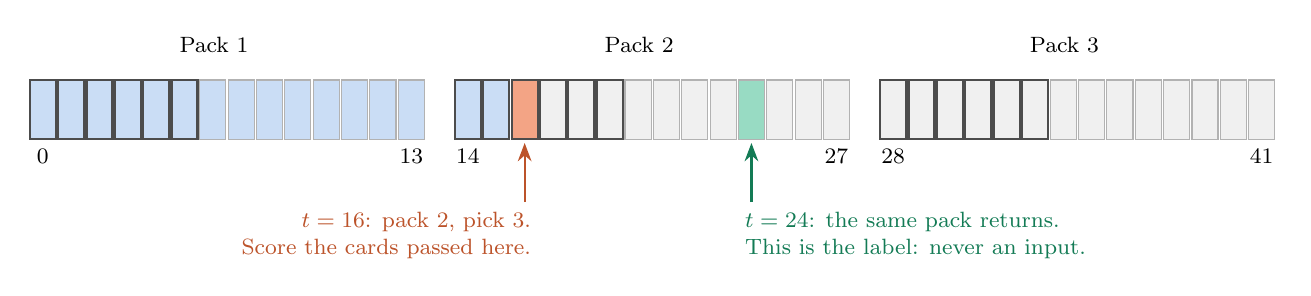
\begin{tikzpicture}[font=\scriptsize,x=0.36cm,y=0.5cm]
\foreach \k/\lab in {0/Pack 1,1/Pack 2,2/Pack 3} {
  \node[font=\footnotesize] at (\k*15+6.5,2.4) {\lab};
  \foreach \i in {0,...,13} {
    \pgfmathtruncatemacro{\t}{\k*14+\i}
    \ifnum\t<16
      \fill[cblue!25] (\k*15+\i,0) rectangle ++(0.92,1.5);
    \else\ifnum\t=16
      \fill[corange!60] (\k*15+\i,0) rectangle ++(0.92,1.5);
    \else\ifnum\t=24
      \fill[caqua!45] (\k*15+\i,0) rectangle ++(0.92,1.5);
    \else
      \fill[black!6] (\k*15+\i,0) rectangle ++(0.92,1.5);
    \fi\fi\fi
    \ifnum\i<6 \draw[black!70,thick] (\k*15+\i,0) rectangle ++(0.92,1.5);
    \else \draw[black!30] (\k*15+\i,0) rectangle ++(0.92,1.5); \fi
  }
}
\node[font=\footnotesize] at (0.46,-0.45) {0};
\node[font=\footnotesize] at (13.46,-0.45) {13};
\node[font=\footnotesize] at (15.46,-0.45) {14};
\node[font=\footnotesize] at (28.46,-0.45) {27};
\node[font=\footnotesize] at (30.46,-0.45) {28};
\node[font=\footnotesize] at (43.46,-0.45) {41};
\draw[corange!80!black,thick,-{Stealth}] (17.46,-1.6) node[below left=0pt and -6pt,align=right,font=\footnotesize]
  {$t=16$: pack 2, pick 3.\\Score the cards passed here.} -- (17.46,-0.1);
\draw[caqua!70!black,thick,-{Stealth}] (25.46,-1.6) node[below right=0pt and -6pt,align=left,font=\footnotesize]
  {$t=24$: the same pack returns.\\This is the label: never an input.} -- (25.46,-0.1);
\end{tikzpicture}
\caption{The 42 slots of one draft. Thick outlines mark the 18 wheel-eligible picks. When scoring the cards
passed at $t=16$ (orange), the model may use every slot up to and including 16 (blue): every pack shown and
every pick made, \emph{including the pick at 16}, since the drafter has already picked when they pass. The
pack shown at $t=24$ (green) is what the model is predicting, so it and everything else after 16 (grey) must be
hidden.}
\label{fig:grid}
\end{figure}

The model processes 128 drafts at a time (a \emph{batch}), so in the code most tensors have a leading
batch dimension $B=128$: \code{pack} is \shape{B, 42, 14}, and so on. Below we usually drop $B$ and talk
about one draft.

\paragraph{One forward pass scores all 234 slots at once.} The model does not run 18 separate times, once per
wheel pick. It reads the whole draft in one go and outputs a probability for every passed card at every
wheel-eligible pick. It can do this without cheating because of two masks (Sections~\ref{sec:causal}
and~\ref{sec:decoder}): the computation for a card passed at $t$ is wired so that it only uses slots $\le t$.
This matters more than usual here, because the answer for pick $t$ is sitting in the data at slot $t+8$.

% =====================================================================
\section{Step 1: turning a card into a vector}\label{sec:cards}

Neural networks work on lists of numbers, so the first job is to give every card a vector of $d=192$
numbers. Think of these as coordinates in a ``card space'' where cards the table treats alike land near each
other. A card's vector is the sum of two parts:

\begin{enumerate}
\item \textbf{A learned vector for the card.} A lookup table with one row of 192 numbers per card (339 for
MSH, plus an empty row). The numbers start random and are tuned during training. Nothing tells the model
what they mean; it discovers, say, that one direction means ``everyone takes this early'' because that helps
it predict what wheels.
\item \textbf{A projection of fixed card attributes.} Each card also has 14 fixed numbers: five colour flags,
a one-hot rarity, mana value (scaled to 0--1), a creature flag and a bonus-sheet flag. A learned
$14\times192$ matrix maps these into the same space, so colour and rarity information is there from the
first training step.
\end{enumerate}

\[
\mathbf{e}_c \;=\; \underbrace{\text{CardEmbedding}[c]}_{\text{learned, per card}}
\;+\; \underbrace{W_{\text{feat}}\,\mathbf{f}_c}_{\text{learned map of fixed attributes}}
\qquad \mathbf{e}_c \in \mathbb{R}^{192}
\]

The whole table, \shape{340, 192}, is computed once per forward pass and then looked up everywhere a card
appears. In the code this is \code{card\_table()}. Section~\ref{sec:multi} describes a variant that drops the
learned row and builds each card from a much richer feature vector, so one model can cover many sets.

\paragraph{A ``bag'' of cards.} Some inputs are a set of cards rather than one card: the pack shown, the
cards the others took. The model turns a set into one vector by taking the \emph{count-weighted average} of
the card vectors, then passing it through a learned $192\times192$ linear layer. This is what the code calls
\code{\_bag()}. A pack with two copies of card A and one of card B becomes
$\tfrac{2}{3}\mathbf{e}_A + \tfrac{1}{3}\mathbf{e}_B$. Averaging throws away order and exact composition,
but keeps the gist: ``this pack is mostly blue, with one strong rare''. Both bags use the same card table
(\code{tied\_bag=True}), each through its own linear layer.

% =====================================================================
\section{Step 2: building one history token per pick}\label{sec:tokens}

The history encoder reads a sequence of 42 \emph{tokens}, one per pick slot. Token $t$ is the \emph{sum} of
five pieces of information, each first mapped into the same 192-number space:

\begin{figure}[!htbp]
\centering
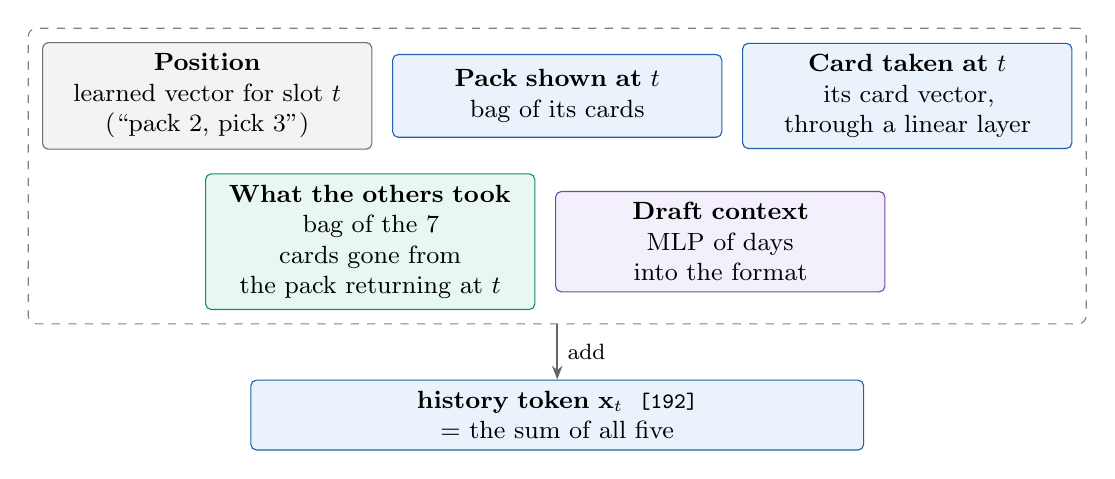
\begin{tikzpicture}[font=\small,
  part/.style={box=#1,text width=3.9cm,minimum height=1.05cm},
  part/.default=cgray]
\node[part] (p1) {\textbf{Position}\\learned vector for slot $t$\\(``pack 2, pick 3'')};
\node[part=cblue,right=0.25cm of p1] (p2) {\textbf{Pack shown at $t$}\\bag of its cards};
\node[part=cblue,right=0.25cm of p2] (p3) {\textbf{Card taken at $t$}\\its card vector,\\through a linear layer};
\node[part=caqua,below=0.3cm of p1,xshift=2.07cm] (p4) {\textbf{What the others took}\\bag of the 7 cards gone from\\the pack returning at $t$};
\node[part=cpurple,right=0.25cm of p4] (p5) {\textbf{Draft context}\\MLP of days into the format};
\node[draw=black!50,dashed,rounded corners=3pt,inner sep=5pt,fit=(p1)(p3)(p4)(p5)] (all) {};
\node[box=cblue,below=0.7cm of all,text width=7.5cm] (tok) {\textbf{history token} $\mathbf{x}_t$ \;\shape{192}\\= the sum of all five};
\draw[arr] (all) -- node[right,font=\footnotesize]{add} (tok);
\end{tikzpicture}
\caption{The five ingredients of history token $t$. Each is mapped to 192 numbers and they are simply
added. Adding (rather than concatenating) is standard in transformers: the network learns to keep the
ingredients in roughly separate directions of the space.}
\label{fig:token}
\end{figure}

\begin{itemize}
\item \textbf{Position.} One learned vector per slot (42 of them). Without it the model would not know
whether a token is pick 1 or pick 14, and wheeling depends heavily on that: a card passed at pick 1 has to
survive seven drafters choosing from a full pack, one passed at pick 6 only from a nearly empty one.
\item \textbf{Pack shown at $t$.} The bag of the cards in front of the drafter.
\item \textbf{Card taken at $t$.} The vector of the card the drafter took \emph{at this same pick}. This is
the most important difference from PickNet, where token $t$ holds the pick at $t-1$ because pick $t$ is the
answer. In WheelNet the question is asked after the drafter has picked, about what they passed, so their
own pick is legitimately known. (The passed cards are the pack shown minus this pick.)
\item \textbf{What the others took.} Explained below; this is the input that lets the model read signals.
\item \textbf{Draft context.} Section~\ref{sec:ctx}.
\end{itemize}

There is no set embedding: a per-set WheelNet only ever sees one set.

\subsection{``What the others took''}

With eight drafters, a pack you see at pick $p$ comes back to you at pick $p+8$, after each of the other
seven has taken one card from it. Comparing the two snapshots tells you exactly which seven cards the
table took, even though the data never says who the other drafters are.

\begin{figure}[!htbp]
\centering
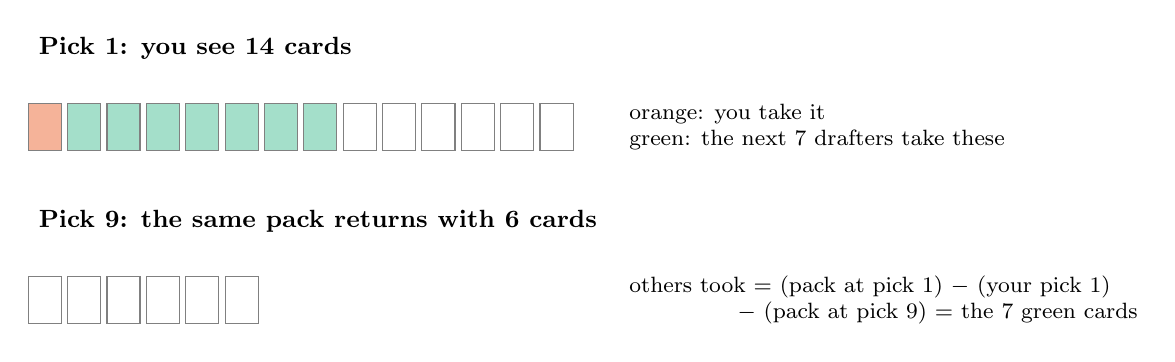
\begin{tikzpicture}[font=\small,
  c/.style={draw=black!50,fill=#1,minimum width=0.42cm,minimum height=0.6cm,inner sep=0pt},
  c/.default=white]
\node[anchor=west,font=\small\bfseries] at (-0.2,1.0) {Pick 1: you see 14 cards};
\foreach \i in {0,...,13} {
  \ifnum\i=0 \node[c=corange!50] at (\i*0.5,0) {}; \else
  \ifnum\i<8 \node[c=caqua!40] at (\i*0.5,0) {}; \else \node[c] at (\i*0.5,0) {}; \fi\fi
}
\node[anchor=west,font=\footnotesize,align=left] at (7.3,0) {orange: you take it\\green: the next 7 drafters take these};
\node[anchor=west,font=\small\bfseries] at (-0.2,-1.2) {Pick 9: the same pack returns with 6 cards};
\foreach \i in {8,...,13} \node[c] at (\i*0.5-4,-2.2) {};
\node[anchor=west,font=\footnotesize,align=left] at (7.3,-2.2)
  {others took $=$ (pack at pick 1) $-$ (your pick 1)\\\hspace{4.6em}$-$ (pack at pick 9) $=$ the 7 green cards};
\end{tikzpicture}
\caption{How ``what the others took'' is computed (\code{taken\_by\_others()} in \code{mtgdata.encode}).
The same subtraction works for every pick from 9 onward in each pack; for picks 1--8 nothing has come back
yet, so this input is zero. The white cards at pick 9 are exactly the cards that wheeled from pick 1.}
\label{fig:others}
\end{figure}

This input is the wheel label of an earlier pick, turned around: token 8 holds the answer to the question
asked at token 0. That is fine, and useful: by the time the model scores pick 2 of pack 2, it knows what wheeled
(and what was taken) from every pack of round 1. If the green cards you passed are all gone but the blue
ones wheel, blue is probably open, and blue cards you pass now are more likely to come back. But it is also
why the masks matter so much: a token from 8 or more slots after the pick being scored would contain its answer.

\subsection{Draft context}\label{sec:ctx}

The shipped model gets two numbers per draft, identical for all 42 tokens: the number of days since the
set's first draft in the data, divided by 30, and $\ln(1+\text{days})/\ln 31$. A small MLP
($2\to192\to192$) turns them into a vector added to every token.

Why the date? Early in a format, drafters haven't settled on which cards are good, so what the table takes,
and so what wheels, keeps moving for weeks. An input ablation on MSH tried each optional input: days into the
format was the only one that helped (validation log loss $-$0.0039). The drafter's rank and 17Lands skill
buckets added nothing, because the drafter's picks already show how they draft, and card types were a
wash. Time is a continuous number rather than a ``which week'' lookup because the test drafts come from the
end of the format, in weeks no training draft covers.

% =====================================================================
\section{Step 3: the history encoder}\label{sec:causal}

Now we have 42 tokens, but each one only knows about its own slot. Token 16 holds pack 16 and pick 16, but
not pick 3. The history encoder's job is to let every token gather information from the earlier ones, so
that the output at slot $t$ summarises the \emph{whole} draft up to $t$. It does this with
\emph{self-attention}.

\subsection{Attention in one paragraph}

Each token computes three vectors from itself: a \emph{query} (``what am I looking for?''), a \emph{key}
(``what do I contain?'') and a \emph{value} (``what do I pass on if you pick me?''). Token $t$ compares its
query with every other token's key; the better the match, the bigger the weight. It then takes the
weighted average of the values and adds it to itself. So token 16 might learn to look hard at the tokens
from round 1 where blue cards wheeled, and pull in ``blue is flowing'' from them. The query, key and value maps are
learned. WheelNet uses 6 \emph{heads}: 6 independent attention patterns run side by side, each on a 32-number
slice of the vector.

A transformer \emph{layer} is one attention step followed by a small per-token MLP ($192\to768\to192$, ReLU),
each wrapped with layer normalisation before it (``pre-norm'') and a residual (``add the result back to the
input'') connection. The history encoder stacks \textbf{4} of these layers (\code{nn.TransformerEncoder}).

\subsection{The causal mask}

If token 16 could attend to token 24, it would see the pack that returns at 24: the answer. The \emph{causal
mask} forbids that: token $t$ may attend only to tokens $0,\dots,t$.

\begin{figure}[!htbp]
\centering
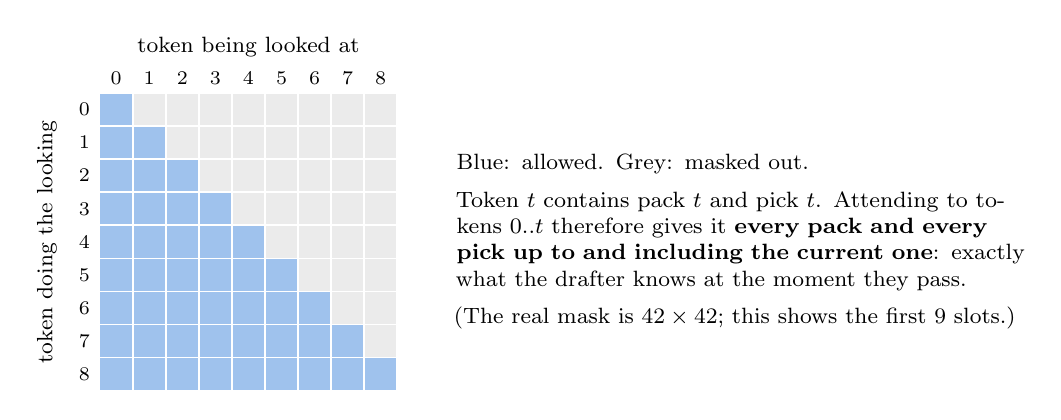
\begin{tikzpicture}[x=0.42cm,y=0.42cm,font=\scriptsize]
\foreach \r in {0,...,8} {
  \foreach \c in {0,...,8} {
    \ifnum\c>\r \fill[black!8] (\c,-\r) rectangle ++(1,-1);
    \else \fill[cblue!45] (\c,-\r) rectangle ++(1,-1); \fi
    \draw[white,line width=0.6pt] (\c,-\r) rectangle ++(1,-1);
  }
  \node[anchor=east] at (0,-\r-0.5) {\r};
  \node at (\r+0.5,0.45) {\r};
}
\node[font=\footnotesize,rotate=90] at (-1.6,-4.5) {token doing the looking};
\node[font=\footnotesize] at (4.5,1.4) {token being looked at};
\node[anchor=west,font=\footnotesize,align=left,text width=7.2cm] at (10.5,-4.5) {
  Blue: allowed. Grey: masked out.\\[4pt]
  Token $t$ contains pack $t$ and pick $t$. Attending to tokens $0..t$ therefore gives it
  \textbf{every pack and every pick up to and including the current one}: exactly what the drafter knows
  at the moment they pass.\\[4pt]
  (The real mask is $42\times42$; this shows the first 9 slots.)};
\end{tikzpicture}
\caption{The causal mask (\code{self.causal}). Because of it, one pass over the whole draft gives 42 honest
states, each blind to everything after its own slot.}
\label{fig:mask}
\end{figure}

The output is one \emph{state} $\mathbf{h}_t$ (192 numbers) per slot, after a final layer normalisation.
$\mathbf{h}_t$ is the model's summary of the draft just after pick $t$. Because of the mask, it is the same
whether you compute it from the full draft or only the first $t+1$ slots; that is what makes the parallel
training legitimate, and it is how you use the model live: feed in the draft so far, read off the last
slot.

Only 18 of the 42 states are used to build passed-card tokens: those at the wheel-eligible slots
$t \in \{0,\dots,5,\;14,\dots,19,\;28,\dots,33\}$ (\code{self.wheel\_pos}). All 42 are available to the
decoder's cross-attention, subject to its own mask.

% =====================================================================
\section{Step 4: passed-card tokens}

The history encoder knows the table; now the model must score the cards the drafter passed. Each distinct
card $c$ passed at wheel pick $t$ gets its own \emph{passed-card token}, again a sum:

\[
\mathbf{z}_{t,c} \;=\; \underbrace{\mathbf{e}_c}_{\text{card vector}}
\;+\; \underbrace{\text{CopiesEmbedding}[\text{copies}_c]}_{\text{1, 2 or 3+ copies}}
\;+\; \underbrace{\text{WheelPickEmbedding}[t]}_{\text{which of the 18}}
\;+\; \underbrace{W_{\text{state}}\,\mathbf{h}_t}_{\text{the table right now}}
\]

So the token ``Super Suit, passed at pack 1 pick 2'' starts out knowing what Super Suit is, that it was passed
at the second pick of round 1, and what the draft looks like at that moment. A pack with two copies of a card
gives \emph{one} token with copies $=2$, matching the label (``at least one copy comes back''). The wheel-pick
embedding is a separate table from the 42 history positions; it tells the decoder how many cards remain to
absorb the seven picks.

Every wheel pick gets up to 13 passed-card slots, so there are $18\times13=234$ tokens per draft,
\shape{234, 192}. Empty slots are masked out. In the code the projection $W_{\text{state}}$ is called
\code{self.ctx}; despite the name it projects the history state, not the draft context.

% =====================================================================
\section{Step 5: the pack decoder}\label{sec:decoder}

The pack decoder refines the passed-card tokens with \textbf{3 blocks} (\code{nn.TransformerDecoder}). Each
block does three things, each with layer normalisation before it and a residual connection around it:

\begin{figure}[!htbp]
\centering
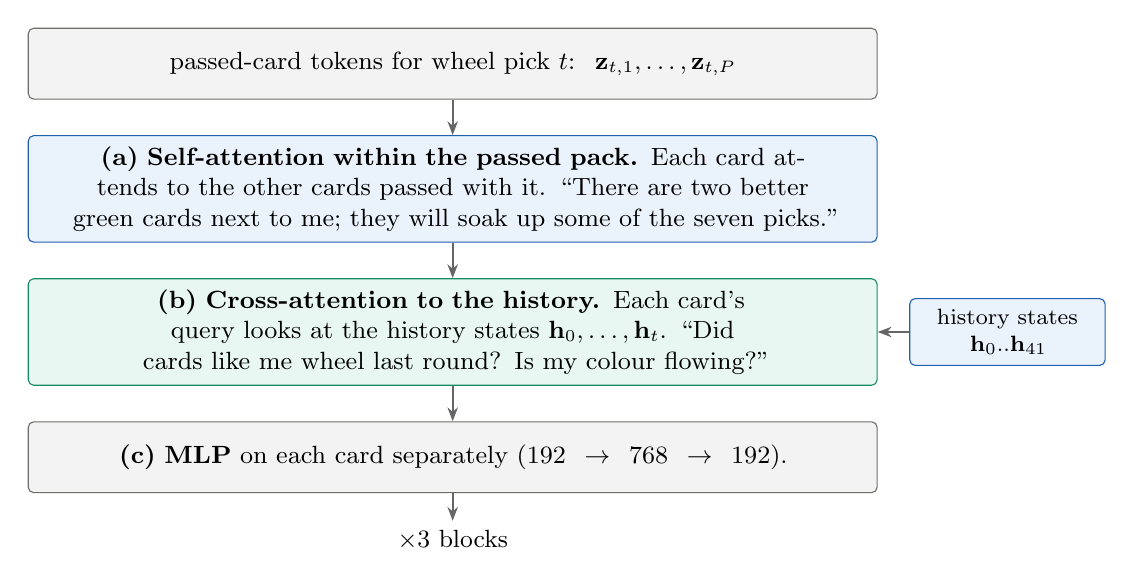
\begin{tikzpicture}[font=\small,node distance=0.45cm,
  st/.style={box=#1,text width=10.5cm,minimum height=0.9cm}]
\node[st=cgray] (in) {passed-card tokens for wheel pick $t$: \;$\mathbf{z}_{t,1},\dots,\mathbf{z}_{t,P}$};
\node[st=cblue,below=of in] (sa) {\textbf{(a) Self-attention within the passed pack.} Each card attends to the
other cards passed with it. ``There are two better green cards next to me; they will soak up some of the seven
picks.''};
\node[st=caqua,below=of sa] (ca) {\textbf{(b) Cross-attention to the history.} Each card's query looks at the
history states $\mathbf{h}_0,\dots,\mathbf{h}_t$. ``Did cards like me wheel last round? Is my colour
flowing?''};
\node[st=cgray,below=of ca] (mlp) {\textbf{(c) MLP} on each card separately ($192\to768\to192$).};
\node[below=0.35cm of mlp,font=\small] (rep) {$\times 3$ blocks};
\draw[arr] (in) -- (sa);
\draw[arr] (sa) -- (ca);
\draw[arr] (ca) -- (mlp);
\draw[arr] (mlp) -- (rep);
\node[box=cblue,right=0.4cm of ca,text width=2.2cm,font=\footnotesize] (h) {history states\\$\mathbf{h}_0..\mathbf{h}_{41}$};
\draw[arr] (h) -- (ca);
\end{tikzpicture}
\caption{One pack-decoder block.}
\label{fig:block}
\end{figure}

\textbf{(a) is why WheelNet beats a per-card statistic.} A card wheels only if the seven drafters after you
all find something they want more. Whether they do depends on what else is in the pack. A decent card passed
alongside two bombs is shielded; the same card as the best thing left is not. ALSA averages this away; the
gradient-boosted baseline in the paper encodes it by hand as \code{n\_better} (how many passed cards usually
go before this one). Self-attention among the passed cards learns it.

\textbf{(b) is how it reads signals.} Here the \emph{passed cards} ask the questions and the \emph{history
states} answer. A card passed at pack 2, pick 3 can pull from any $\mathbf{h}_s$ with $s\le16$, including
the round-1 states that saw what came back.

\subsection{Two masks}

All 18 passed packs of a draft are laid out as one sequence of 234 tokens, so the history is projected into
keys and values once per draft instead of once per pack. Two masks keep this honest:

\begin{figure}[!htbp]
\centering
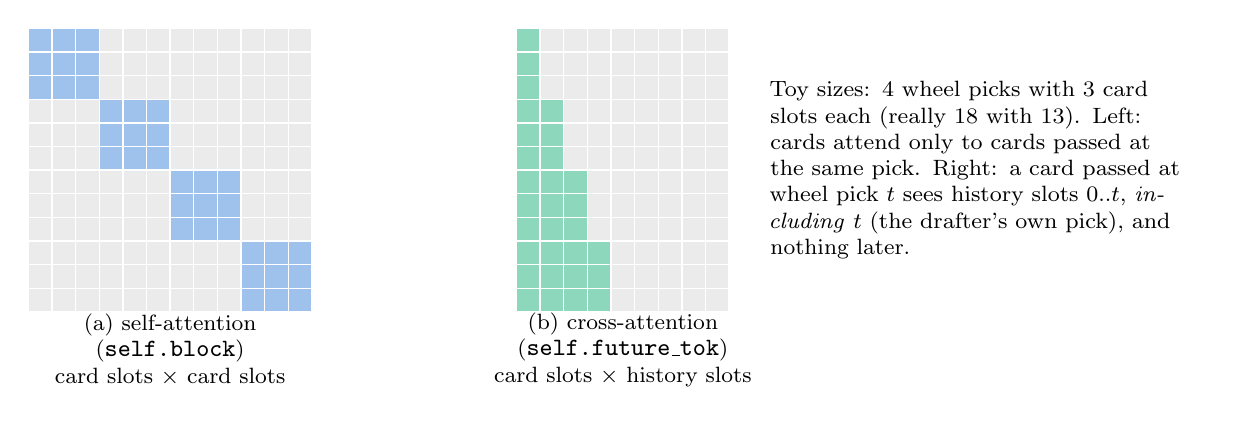
\begin{tikzpicture}[x=0.3cm,y=0.3cm,font=\scriptsize]
% left: block-diagonal self-attention, 4 packs of 3 slots
\foreach \r in {0,...,11} {
  \foreach \c in {0,...,11} {
    \pgfmathtruncatemacro{\br}{\r/3}\pgfmathtruncatemacro{\bc}{\c/3}
    \ifnum\br=\bc \fill[cblue!45] (\c,-\r) rectangle ++(1,-1);
    \else \fill[black!8] (\c,-\r) rectangle ++(1,-1); \fi
    \draw[white,line width=0.5pt] (\c,-\r) rectangle ++(1,-1);
  }
}
\node[font=\footnotesize,align=center] at (6,-13.6) {(a) self-attention\\(\code{self.block})\\card slots $\times$ card slots};
% right: cross-attention, 4 wheel picks x 9 history slots
\begin{scope}[xshift=6.2cm]
\foreach \r in {0,...,11} {
  \pgfmathtruncatemacro{\w}{\r/3}
  \foreach \c in {0,...,8} {
    \ifnum\c>\w \fill[black!8] (\c,-\r) rectangle ++(1,-1);
    \else \fill[caqua!50] (\c,-\r) rectangle ++(1,-1); \fi
    \draw[white,line width=0.5pt] (\c,-\r) rectangle ++(1,-1);
  }
}
\node[font=\footnotesize,align=center] at (4.5,-13.6) {(b) cross-attention\\(\code{self.future\_tok})\\card slots $\times$ history slots};
\end{scope}
\node[anchor=west,font=\footnotesize,text width=5.4cm] at (31,-6) {Toy sizes: 4 wheel picks with 3 card slots
each (really 18 with 13). Left: cards attend only to cards passed at the same pick. Right: a card passed at
wheel pick $t$ sees history slots $0..t$, \emph{including} $t$ (the drafter's own pick), and nothing later.};
\end{tikzpicture}
\caption{The pack decoder's masks. The real ones are $234\times234$ and $234\times42$.}
\label{fig:dmask}
\end{figure}

One edge case: a few sets' files lack pack 1, pick 1, so that wheel pick has no passed cards. A token with
nothing to attend to produces NaNs, so the code lets an all-empty pack attend to its first padding slot.
Those outputs are never scored.

% =====================================================================
\section{Step 6: from scores to probabilities}\label{sec:softmax}

After the last block, a small head (layer norm, $192\to192$, GELU, $192\to1$) turns each passed-card token into
a single number, its \emph{logit}. The probability that card $c$ comes back is the sigmoid of its logit:
\[
P(c \text{ wheels} \mid \text{everything so far}) \;=\; \sigma(\text{logit}_c) \;=\; \frac{1}{1+e^{-\text{logit}_c}}.
\]
This is \emph{not} a softmax. PickNet's question has exactly one answer per pack (the card the human took),
so its probabilities sum to 1. Here several cards can come back, and each gets its own yes/no probability.
The loss is the binary cross-entropy of each real passed card, averaged over all of them:
\[
\text{loss} = -\frac{1}{N}\sum_{\text{passed cards}} \Big[\, y\,\ln p + (1-y)\ln(1-p) \,\Big].
\]

\paragraph{A worked example.} A real MSH test draft (from the QA section of \code{notebooks/wheel.ipynb}),
pack 1, pick 2, drafted on day 23 of the format. The drafter was shown 13 cards and passed 12. Five come back
at pick 10.

\begin{center}\small
\begin{tabular}{lccc l}
\toprule
card passed & P(wheel) & came back? & loss (nats) & \\
\midrule
Island & 0.996 & yes & 0.004 & \textcolor{cblue}{\rule{2.99cm}{6pt}} \\
Hex Magic & 0.877 & yes & 0.131 & \textcolor{cblue}{\rule{2.63cm}{6pt}} \\
Volcanic Villain & 0.841 & \textbf{no} & 1.839 & \textcolor{cgray}{\rule{2.52cm}{6pt}} \\
Kingpin's Enforcers & 0.573 & yes & 0.557 & \textcolor{cblue}{\rule{1.72cm}{6pt}} \\
Super Suit & 0.495 & yes & 0.703 & \textcolor{cblue}{\rule{1.49cm}{6pt}} \\
Mockingbird, Ace Agent & 0.315 & no & 0.378 & \textcolor{cgray}{\rule{0.95cm}{6pt}} \\
Wakandan Drone Flock & 0.253 & no & 0.292 & \textcolor{cgray}{\rule{0.76cm}{6pt}} \\
Pet Avengers & 0.240 & no & 0.274 & \textcolor{cgray}{\rule{0.72cm}{6pt}} \\
Beast, Erudite Aerialist & 0.203 & \textbf{yes} & 1.595 & \textcolor{cblue}{\rule{0.61cm}{6pt}} \\
Jessica Jones, Private Eye & 0.065 & no & 0.067 & \textcolor{cgray}{\rule{0.20cm}{6pt}} \\
Titania, Rugged Rumbler & 0.047 & no & 0.048 & \textcolor{cgray}{\rule{0.14cm}{6pt}} \\
S.H.I.E.L.D. Spy Kit & 0.044 & no & 0.045 & \textcolor{cgray}{\rule{0.13cm}{6pt}} \\
\midrule
sum / mean & 4.95 & 5 & 0.494 & \\
\bottomrule
\end{tabular}
\end{center}

\begin{itemize}
\item \textbf{Loss}: each card's loss is $-\ln p$ if it came back and $-\ln(1-p)$ if not. The two surprises,
Volcanic Villain (taken at 84\%) and Beast (back at 20\%), cost 1.8 and 1.6 nats; the confident right calls
cost almost nothing. This pack averages 0.494 nats per card; the model averages 0.422 over the MSH test set.
\item \textbf{Expected count}: the probabilities sum to 4.95, and 5 cards came back. With 13 cards and 8
drafters, exactly $13-8=5$ cards return to this pick, but the model is never told that. Averaged over the
test set the sum matches the true count at every pick (6.02 vs 6.00 at pick 1 \ldots\ 0.99 vs 1.00 at pick 6),
which is good evidence it has learned how a table behaves, not just per-card rates.
\item \textbf{Calibration}: because the loss punishes confident mistakes, the probabilities can be read at
face value. Of the second-best cards drafters pass that WheelNet gives 30--50\%, a third come back.
\end{itemize}

% =====================================================================
\section{The features-only variant: one model for many sets}\label{sec:multi}

The per-set model has a learned row for each card, so it can only score a set it was trained on. With
\code{ids=False} the learned row goes away, and a card is \emph{only} a function of its features:

\[
\mathbf{e}_c \;=\; \text{MLP}(\mathbf{f}_c), \qquad \text{MLP}: 465 \to 384 \xrightarrow{\text{GELU}} 192.
\]

$\mathbf{f}_c$ has 465 numbers: the 14 attributes above, card types and supertypes, Scryfall-derived rules
features (power and toughness, keywords, mana production, rules-text roles), and a 384-number embedding of
the rules text from the small language model \code{bge-small-en-v1.5}, as in PickNet. The features are
standardised over all cards of all training sets. Because every card is described in the same terms, one set
of weights scores any set, including cards it has never seen.

Everything else is unchanged, except that this variant uses the full draft context: rank (7 numbers),
17Lands skill buckets (4) and the two time numbers, 13 in all. The card table of the 8 training sets has
2,573 rows, and each set's local card ids are shifted into it (\code{remap()} in
\code{train\_wheelnet\_multiset.py}). It has 4,051,009 parameters: the card MLP's 252,864 replace the per-set
model's 67,968.

Trained on 20k drafts from each of 7 other sets plus MSH's own training drafts, it is the best MSH model
(test log loss 0.4188, against 0.4218 for the shipped per-set model). Without MSH's drafts it scores 0.5245:
it knows how tables behave but not which of a new set's cards are good.

% =====================================================================
\section{Training}

\begin{itemize}
\item \textbf{Data.} MSH's first 70\% of drafts by time: 48,026 drafts, 9.1M passed cards. Each batch is 128
drafts, about 24,000 passed cards per update.
\item \textbf{Loss.} Mean binary cross-entropy over every real passed card.
\item \textbf{Optimiser.} AdamW (weight decay 0.01), gradients clipped at norm 1, a one-cycle learning-rate
schedule: 5\% linear warm-up to $10^{-3}$, then a cosine decay to near zero.
\item \textbf{Epochs.} 8 on MSH (3,008 steps, about 26 minutes on an Apple-silicon laptop). Other sets get
$\mathrm{round}(8 \cdot 48\text{k} / \text{training drafts})$, clamped to 3--8, so every set costs about the
same.
\item \textbf{Early stopping.} After each epoch the model is scored on the validation drafts (the next 15\% by
time); the best epoch's weights are kept. The test drafts (the last 15\%) are scored once, at the end.
\item \textbf{Regularisation.} Dropout 0.2 throughout. At 0.1 the model overfit after epoch 5.
\end{itemize}

\paragraph{Keeping it current.} A model frozen after a format's first week falls behind a weekly retrain by
0.011 log loss by week 5, more than WheelNet's whole lead over the GBM baseline. Fine-tuning the previous
week's model for 2 epochs on the newest week, at learning rate $3\times10^{-4}$, stays within about 0.001 of a
full retrain (\code{scripts/temporal.py}).

% =====================================================================
\section{Shapes and sizes}

Tensor shapes through one forward pass, for a batch of $B=128$ MSH drafts ($T=42$ slots, 18 wheel picks,
13 passed-card slots, $d=192$):

\begin{center}\small
\resizebox{\textwidth}{!}{\begin{tabular}{lll}
\toprule
stage & shape & code \\
\midrule
card table & \shape{340, 192} & \code{card\_table()} \\
pack bag, taken card, others bag, position & \shape{B, 42, 192} each & \code{\_bag(...)}, \code{taken}, \code{self.pos} \\
draft context & \shape{B, 1, 192}, broadcast to all 42 & \code{draft\_ctx} \\
history tokens $\mathbf{x}$ & \shape{B, 42, 192} & \code{h} before \code{self.hist} \\
history states $\mathbf{h}$ & \shape{B, 42, 192} & \code{h} after \code{hist\_norm} \\
wheel states & \shape{B, 18, 192} & \code{h[:, self.wheel\_pos]} \\
passed-card tokens $\mathbf{z}$ & \shape{B, 234, 192} & \code{x} \\
\quad (a) self-attention & block-diagonal, 13 slots per pack & \code{tgt\_mask=self.block} \\
\quad (b) cross-attention & 234 queries per draft over 42 states & \code{memory\_mask=self.future\_tok} \\
logits & \shape{B, 3, 6, 13} & \code{self.head(x)} \\
\bottomrule
\end{tabular}}
\end{center}

Where the 3.86M parameters are:

\begin{center}\small
\begin{tabular}{lrr}
\toprule
component & parameters & share \\
\midrule
card table (339 card vectors + empty row, attribute projection) & 67,968 & 2\% \\
history encoder (4 transformer layers + final norm) & 1,779,840 & 46\% \\
pack decoder (3 blocks) & 1,780,416 & 46\% \\
token input layers (pack, taken, others, context, position) & 156,864 & 4\% \\
passed-card inputs (state projection, copies, wheel pick) and scoring head & 78,913 & 2\% \\
\midrule
total & 3,864,001 & \\
\bottomrule
\end{tabular}
\end{center}

Compared with PickNet, the card table is tiny (one set, 192 dimensions), and almost all the weights are in the
two attention stacks.

% =====================================================================
\section{Putting it together: one wheel pick, start to finish}

Say we want the model's prediction for the cards a drafter passes at pack 2, pick 3 ($t=16$) of MSH, on day
23 of the format.

\begin{enumerate}
\item \textbf{Look up card vectors} for every card that appears anywhere in the draft so far.
\item \textbf{Build tokens 0--16.} Token 16 = position 16 + bag(the 12 cards they were shown) + the card they
took at this pick + context(day 23). Token 16 has no ``others took'' input yet (pack 2 hasn't come round), but
tokens 8--13 do: they hold what the table took from each of round 1's first six packs.
\item \textbf{Run the history encoder.} Four layers of causal attention. State $\mathbf{h}_{16}$ now reflects
all 17 picks so far, every pack they saw, and what wheeled in round 1.
\item \textbf{Build 11 passed-card tokens}, one per card left in the pack: card vector + copies + wheel-pick
embedding for ``pack 2, pick 3'' + projected $\mathbf{h}_{16}$.
\item \textbf{Run the pack decoder.} In each of 3 blocks the 11 cards compare themselves with each other,
consult $\mathbf{h}_0..\mathbf{h}_{16}$, and pass through an MLP.
\item \textbf{Score.} Eleven logits, eleven sigmoids: one probability per card that it is still there at pick 11.
Exactly $14-10=4$ cards return, so their sum should be close to 4.
\end{enumerate}

In training, steps 1--6 happen for all 18 wheel picks and all 128 drafts in the batch at once, and the losses
from all real passed cards are averaged before each update.

% =====================================================================
\section{How WheelNet differs from PickNet}\label{sec:vs}

The two models share a design and most of their code ideas, so the differences are easy to miss.

\begin{center}\small
\begin{tabular}{>{\raggedright}p{3.4cm}>{\raggedright}p{5.2cm}p{5.2cm}}
\toprule
 & PickNet & WheelNet \\
\midrule
question & which card does the drafter take at $t$? & which passed cards come back at $t+8$? \\
scored picks & all 45 slots & the 18 wheel-eligible slots \\
history token $t$ holds & pack $t$, pick $t-1$ & pack $t$, pick $t$ \\
decoder sees history & $\mathbf h_0..\mathbf h_t$ (before pick $t$) & $\mathbf h_0..\mathbf h_t$ (after pick $t$) \\
decoder tokens & every card in pack $t$ & every card passed at $t$ \\
output & softmax over the pack & independent sigmoid per card \\
loss & pick NLL $+\,0.3\times$ deck BCE & BCE per passed card \\
extra heads & deck head & none \\
set embedding & yes (17 sets) & no (per-set); features-only variant for many sets \\
draft context & rank, skill, time, format, pack size & time only (shipped) \\
size & $d=256$, 8 heads, 8.4M params & $d=192$, 6 heads, 3.9M params \\
dropout & 0.05 & 0.2 \\
\bottomrule
\end{tabular}
\end{center}

\noindent The one to watch if you combine them: PickNet's state at $t$ has not seen pick $t$, and
WheelNet's has. A wheel head on a PickNet trunk must add the pick at $t$ itself, and must never attend to slot
$t+8$ or later, which holds the answer. \code{paper/combined/architecture.tex} describes such a shared-trunk version.

% =====================================================================
\section{FAQ}

\paragraph{Why not just use ALSA?} ALSA is a per-card average over every pack a card appeared in. It knows
nothing about what else is in your pack or what your table has been taking. On MSH, WheelNet cuts log loss by
8--9\% against an ALSA-based model, and by 14\% on the best card you pass, where ALSA is badly overconfident.

\paragraph{Does the model know who the other drafters are?} No. It only sees which cards vanished from the
packs that came back. It has to infer what the table is drafting from that.

\paragraph{Why one token per distinct card, not per copy?} The label is ``does at least one copy come
back''. Two copies of a common are one question, with a better chance of an answer of yes; the copies
embedding tells the model there are two.

\paragraph{Can it score picks 7 and later?} No. A pack passed at pick 7 or later of a 14-card round never
returns with cards in it, so there is nothing to predict.

\paragraph{Does it know the drafter's skill?} The shipped model doesn't, by design: rank and skill inputs
didn't help, because what the model needs is how the \emph{table} drafts, and the history already shows it.

\paragraph{Can it predict a set it has never seen?} Only the features-only variant can, and not well: on day
zero it is far behind an ALSA model fitted on a few days of the new set's data.

\end{document}
